% Provenance (never printed): old premiere S material on the history of plate
% tectonics (from continental drift to seafloor spreading: the ridges, the
% magnetic stripes, the ages of the drilled floor); see
% sources/book2/PROVENANCE.md. Profiles are computed in
% figdata/grade-11/magnetic_stripes.py, the age map in seafloor_age.py, the
% drilling fit in sediment_ages.py.
\chapter{De la deriva continental a la expansión del fondo oceánico}\label{ch:g11:drift-to-spreading}

A principios de los años cincuenta, en el laboratorio Lamont de la
Universidad de Columbia, una joven geóloga llamada Marie Tharp estaba sentada ante largas filas de números. Cada uno era una
profundidad del Atlántico Norte, medida por la ecosonda de un barco, una
detrás de otra a lo largo de la derrota del barco. Representándolas una a
una, dibujó la forma del fondo oceánico a lo largo de las derrotas de barcos
que habían cruzado el océano. En el centro del océano el fondo se elevaba en
una cordillera --- y en todas las derrotas, a lo largo de la cresta de la
cordillera, el fondo volvía a hundirse en una hendidura profunda, como si las
montañas se hubieran partido por la mitad. Este capítulo sigue cómo esas
medidas del fondo oceánico convirtieron una idea rechazada, la deriva de los
continentes, en una teoría: el fondo oceánico se fabrica en las dorsales y se
aleja de ellas, y lleva en sus rocas un registro de su propia edad.
% ledger: aip:tharp, aip:featureless, usgs:echo-sounding

\begin{recall}
La deriva continental es la idea de que los continentes se mueven; Alfred
Wegener la defendió desde 1912 con el encaje de las costas, los fósiles, las
rocas y los climas antiguos, pero no supo decir qué los movía. La superficie
de la Tierra está formada por placas rígidas, que se encuentran en límites
divergentes, convergentes y transformantes; se mueven unos centímetros al
año, y $\qty{1}{cm}$ al año son $\qty{10}{km}$
por millón de años (Libro 1, año 7). El fondo oceánico tiene su plataforma
continental, sus llanuras abisales, sus dorsales y sus fosas (Libro 1,
año 8). La Tierra tiene un campo magnético, con un polo norte y un polo sur
magnéticos, que sigue la aguja de una brújula; un impulso sonoro enviado al
agua vuelve como eco al cabo de un tiempo que da la distancia (los libros de
física).
\end{recall}

\section{Por qué se rechazó la deriva}

Las pruebas de Wegener mostraban que los continentes habían estado unidos. Lo
que no mostraban era cómo podían haberse movido. Wegener imaginaba los
continentes abriéndose paso a través de la roca del fondo oceánico, y los físicos respondieron que ninguna fuerza conocida podía empujar un continente a través de roca sólida
sin aplastarlo. Durante medio siglo, la mayoría de los geólogos concluyeron
que los continentes no se habían movido en absoluto.
% ledger: usgs:wegener-1912, usgs:jeffreys (Book 1 rows)

Faltaban dos cosas. La primera era un mecanismo. La segunda, que llevó a la
primera, era conocer el fondo de los océanos, que cubre la mayor parte de la
superficie de la Tierra y que, en 1912, casi nadie había visto: se suponía que
era una llanura casi sin relieve.
% ledger: aip:tharp, aip:featureless

\section{Cartografiar el fondo oceánico}

Una ecosonda envía un breve impulso sonoro desde el casco de un barco hasta
el fondo marino y mide el tiempo que tarda su eco. El sonido viaja por el agua
de mar a unos \qty{1500}{m/s}; el impulso baja y vuelve, así que un retraso
$t$ corresponde a una profundidad
\[
  d = \frac{v\,t}{2}.
\]
Un retraso de \qty{6.0}{s}, por ejemplo, corresponde a $1500 \times 6.0/2 =
\qty{4500}{m}$ de agua. En el siglo XIX, las profundidades se medían de una
en una, bajando hasta el fondo un cabo lastrado. Después de la Primera Guerra
Mundial se impusieron las ecosondas, y los registros de sus ecos mostraron un
fondo mucho más accidentado de lo que nadie había pensado; en los años cincuenta, campañas de barcos de muchos países mostraron que una
gran cordillera del fondo oceánico da casi la vuelta entera a la
Tierra.
% ledger: noaa:sound-seawater, usgs:echo-sounding, usgs:line-soundings

\begin{history}[Marie Tharp y el valle de rift, 1952]
% ledger: aip:tharp, aip:featureless
Desde 1947, el geofísico Bruce Heezen había reunido perfiles de ecosonda a
través del Atlántico Norte. Marie Tharp, a quien entonces no se le permitía
embarcar en los buques oceanográficos, convirtió lo que más tarde llamó
``interminables filas de números de sondeo'' en dibujos del fondo marino. En
1952, con las derrotas este--oeste ordenadas de norte a sur, vio que un rasgo
se alineaba de una derrota a otra: una hendidura a lo largo de la cresta de
la dorsal mesoatlántica, un valle de rift. Heezen pensó al principio que era
un error. Después se comprobó que los epicentros de los terremotos del
Atlántico, representados a la misma escala, caían en el propio valle de rift.
El mapa del fondo oceánico mundial de Tharp y Heezen,
pintado por el artista Heinrich Berann en 1977, dio a la gente la primera imagen realista del fondo oceánico; en 1997 la
Biblioteca del Congreso la nombró una de las cuatro grandes cartógrafas del
siglo XX.
\end{history}

Las dorsales oceánicas forman un único sistema casi continuo de unos
\qty{65000}{km} de longitud, sumergido en más de sus nueve décimas partes; la
cresta está de media a \qty{2500}{m} por debajo de la superficie. A lo largo
de la lenta dorsal mesoatlántica, la cresta está cortada por un valle de
rift; a lo largo de la dorsal del Pacífico oriental, más rápida, es una cima
suave y redondeada. Los terremotos de los océanos siguen de cerca las
dorsales. Todo señalaba la dorsal como un lugar
donde algo estaba ocurriendo --- pero ¿qué?
% ledger: noaa:ridge, aip:tharp

\section{La expansión del fondo oceánico}

\begin{history}[Hess y la cinta transportadora, 1962]
% ledger: usgs:hess, hess:1962
En 1962, Harry Hess, geólogo de la Universidad de Princeton y almirante de la
reserva naval, publicó \emph{History of Ocean Basins}.
Propuso que la roca caliente sube bajo las dorsales y se convierte en fondo
oceánico nuevo, que después se aleja hacia ambos lados como una cinta
transportadora y vuelve a hundirse en el manto en las fosas. Robert Dietz,
que llegó a la misma idea, le dio su nombre: la \omterm{def:g11:drift-to-spreading:spreading}{expansión del fondo oceánico}.
La idea explicaba por qué la Tierra no crece aunque sin cesar se fabrique
fondo nuevo, por qué hay tan poco sedimento sobre el fondo oceánico y por qué
las rocas del fondo oceánico son mucho más jóvenes que las de los
continentes.
\end{history}

\begin{definition}[Expansión del fondo oceánico]\label{def:g11:drift-to-spreading:spreading}
La \emph{expansión del fondo oceánico}\index{expansion del fondo oceanico@expansión del fondo oceánico}
es el proceso por el que se forma fondo oceánico nuevo a lo largo de la
cresta de una dorsal oceánica, donde la roca fundida sube del manto y se
solidifica, y después se aleja de la dorsal hacia ambos lados, de modo que el
fondo oceánico es más antiguo cuanto más lejos está de la dorsal.
\end{definition}

\begin{definition}[Velocidad de expansión]\label{def:g11:drift-to-spreading:spreading-rate}
La \emph{velocidad de expansión total}\index{velocidad de expansion@velocidad de expansión}
de una dorsal es la velocidad a la que se separan las dos placas situadas a
uno y otro lado de ella. La \emph{semivelocidad de expansión} es la velocidad
a la que el fondo de un lado se aleja del eje de la dorsal. Cuando la
expansión es simétrica, la velocidad total es el doble de la semivelocidad.
\end{definition}

Las dorsales se expanden a velocidades muy distintas. La dorsal mesoatlántica
se abre a razón de \qtyrange{2}{5}{cm} al año; la dorsal del Pacífico
oriental, a razón de \qtyrange{6}{16}{cm} al año. Del fondo oceánico que
existe hoy, alrededor de un tercio se formó en dorsales lentas (velocidades
totales de \qtyrange{20}{55}{mm} al año) y unas dos quintas partes en dorsales
rápidas (\qtyrange{75}{180}{mm} al año).
% ledger: noaa:ridge, seton:rate-classes

La idea de Hess era audaz y, al principio, tenía pocas pruebas directas. Las
pruebas llegaron por dos lados inesperados: el magnetismo del fondo oceánico
y sus sedimentos.

\section{Las inversiones magnéticas y el fondo marino a bandas}

\subsection{Una roca recuerda el campo}

El basalto del fondo oceánico contiene pequeños granos de magnetita, un óxido
de hierro fuertemente magnético. Cuando la lava basáltica sale, está
demasiado caliente para conservar ninguna magnetización duradera; al
enfriarse, los granos se magnetizan paralelamente al campo terrestre que los
rodea, y esa dirección queda entonces fijada en la roca.
% ledger: usgs:magnetometers

\begin{definition}[Magnetización remanente; temperatura de Curie]\label{def:g11:drift-to-spreading:remanence}
La \emph{temperatura de Curie}\index{temperatura de Curie} de un mineral
magnético es la temperatura por encima de la cual no puede conservar una
magnetización propia: unos \qty{580}{\celsius} en la magnetita. Una roca cuyos
granos magnéticos se enfrían por debajo de su temperatura de Curie dentro del
campo terrestre conserva una magnetización paralela al campo de esa época, la
\emph{magnetización remanente}\index{magnetizacion remanente@magnetización remanente}. Dura mucho después de que el campo haya cambiado, salvo que
la roca vuelva a calentarse por encima de la temperatura de Curie.
\end{definition}
% ledger: tarduno:curie

\begin{omfigure}
\begin{tikzpicture}[font=\footnotesize, >={Stealth[length=5pt]}]
  % ground and lava flow
  \fill[lith basalt] (0,0) rectangle (11,0.6);
  \fill[omLithBasalt!45!red!35] (0,0.6) -- (11,0.6) -- (11,1.9) .. controls (9,2.0) and (4,2.15) .. (0,2.05) -- cycle;
  \fill[omLithBasalt!70] (0,1.35) -- (11,1.25) -- (11,1.9) .. controls (9,2.0) and (4,2.15) .. (0,2.05) -- cycle;
  \draw[black!60] (0,1.35) -- (11,1.25);
  \draw[line width=0.8pt] (0,2.05) .. controls (4,2.15) and (9,2.0) .. (11,1.9);
  \draw[black!60] (0,0.6) -- (11,0.6);
  % field lines (northern hemisphere: pointing down to the north)
  \foreach \x in {0.6,2.4,4.2,6.0,7.8,9.6} {
    \draw[->, omDef, line width=0.9pt] (\x,4.0) -- (\x+1.1,2.55);
  }
  \node[anchor=south west, text=omDef] at (0.2,4.05) {el campo magnético de la Tierra};
  % locked grains in the cooled top
  \foreach \x in {0.5,1.3,...,10.5} {
    \draw[->, black, line width=0.6pt] (\x,1.86) -- (\x+0.25,1.53);
  }
  % random grains in the hot interior
  \foreach \x/\a in {0.6/20,1.5/140,2.3/250,3.2/80,4.0/310,4.9/190,5.7/40,6.6/120,7.4/280,8.3/20,9.1/200,10.0/330} {
    \draw[->, black!55, line width=0.5pt] (\x,0.95) -- ++(\a:0.22);
  }
  \node[anchor=west, align=left] at (11.15,1.75) {bajo \qty{580}{\celsius}: los granos\\fijan la dirección del campo};
  \node[anchor=west, align=left] at (11.15,0.92) {todavía por encima de \qty{580}{\celsius}:\\sin magnetización duradera};
  \node[anchor=west, align=left] at (11.15,0.25) {roca más antigua};
  \node[anchor=west] at (9.0,4.25) {norte $\rightarrow$};
\end{tikzpicture}

{\small Una colada de lava que se enfría (esquema, hemisferio norte, donde el
campo apunta hacia el norte y hacia abajo). La parte alta de la colada se ha
enfriado por debajo de la \omterm{def:g11:drift-to-spreading:remanence}{temperatura de Curie} de la magnetita: sus granos
magnéticos (flechas negras) conservan la dirección del campo. El interior,
todavía más caliente, aún no registra nada; registrará el campo del momento
en que se enfríe.}
\end{omfigure}

\subsection{El campo se invierte}

A principios del siglo XX, Bernard Brunhes (en 1906) y después Motonori
Matuyama (en los años veinte) descubrieron que las rocas volcánicas se
reparten en dos grupos. En unas, la magnetización apunta en el mismo sentido
que el campo actual; en las otras apunta en sentido contrario, como si los
polos norte y sur magnéticos se hubieran intercambiado. El propio campo se
había invertido, una y otra vez.
% ledger: usgs:reversals

\begin{definition}[Inversión magnética; polaridad normal e inversa]\label{def:g11:drift-to-spreading:reversal}
Una \emph{inversión magnética}\index{inversion magnetica@inversión magnética}
es un intercambio de los polos norte y sur magnéticos de la Tierra. Una época
en la que el campo apuntaba como hoy es una época de \emph{polaridad
normal}\index{polaridad normal}; una época en la que apuntaba en sentido
contrario, una época de \emph{polaridad
inversa}\index{polaridad inversa}. Una roca magnetizada durante una u otra
época tiene la misma polaridad.
\end{definition}

Las lavas datadas dan la sucesión de intervalos normales e inversos: la
\emph{escala de tiempo de polaridad geomagnética}. Sus intervalos largos
llevan el nombre de científicos que estudiaron el magnetismo terrestre
(Brunhes, Matuyama, Gauss, Gilbert); los episodios cortos que contienen, el
de los lugares donde se descubrieron.

\begin{omfigure}
\begin{tikzpicture}
\begin{axis}[width=0.92\linewidth, height=3.2cm, xmin=0, xmax=5.5, ymin=-0.9, ymax=1.9,
  axis y line=none, axis x line*=bottom, xtick={0,0.5,...,5.5}, tick label style={font=\small},
  xlabel={edad (millones de años)}, label style={font=\small}, clip=false]
\addplot[fill=black, draw=none] table {figdata/out/grade-11-magnetic_stripes-timescale.dat};
\draw[black] (axis cs:0,0) rectangle (axis cs:5.5,1);
\begin{scope}[every node/.style={font=\scriptsize, anchor=south}]
  \node at (axis cs:0.39,1.05) {Brunhes};
  \node at (axis cs:1.68,1.05) {Matuyama};
  \node at (axis cs:3.08,1.05) {Gauss};
  \node at (axis cs:4.74,1.05) {Gilbert};
\end{scope}
\draw[black!60] (axis cs:0.78,1) -- (axis cs:0.78,1.45);
\draw[black!60] (axis cs:2.581,1) -- (axis cs:2.581,1.45);
\draw[black!60] (axis cs:3.58,1) -- (axis cs:3.58,1.45);
\begin{scope}[every node/.style={font=\scriptsize, anchor=north}]
  \node at (axis cs:1.03,-0.05) {Jaramillo};
  \node at (axis cs:1.86,-0.05) {Olduvai};
\end{scope}
\node[font=\scriptsize, anchor=west] at (axis cs:5.55,0.75) {normal};
\node[font=\scriptsize, anchor=west] at (axis cs:5.55,0.25) {(negro)};
\end{axis}
\end{tikzpicture}

{\small La escala de tiempo de polaridad geomagnética de los últimos 5.5
millones de años: en negro, la \omterm{def:g11:drift-to-spreading:reversal}{polaridad normal}; en blanco, la inversa. El
intervalo normal actual empezó hace \num{780000} años; hubo veinte inversiones
en los últimos cinco millones de años. Datos: Cande y Kent (1995).}
\end{omfigure}
% ledger: ck95:chrons

\subsection{Bandas en el fondo oceánico}

A partir de los años cincuenta, los barcos remolcaron magnetómetros a través
de los océanos y descubrieron que el campo en la superficie del mar no era el
campo regular que se esperaba del núcleo terrestre: era un poco más intenso
aquí, un poco más débil allá.
% ledger: usgs:magnetometers

\begin{definition}[Anomalía magnética]\label{def:g11:drift-to-spreading:anomaly}
En un punto de la superficie del mar, la
\emph{anomalía magnética}\index{anomalia magnetica@anomalía magnética} es la intensidad medida del campo magnético menos la intensidad
que cabría esperar allí solo por el campo terrestre. Es positiva donde las
rocas de debajo se suman al campo, y negativa donde se oponen a él. Es pequeña
comparada con el propio campo, y se mide en nanoteslas (\unit{nT}).
\end{definition}

Cartografiadas sobre una región amplia, las anomalías dibujaron bandas
paralelas a la cresta de la dorsal, alternativamente positivas y negativas,
como el pelaje de una cebra --- y el dibujo de un lado de la dorsal era la
imagen especular del dibujo del otro lado.
% ledger: usgs:magnetometers

\begin{history}[Vine y Matthews, 1963]
% ledger: vm:1963, usgs:magnetometers
En septiembre de 1963, Fred Vine y Drummond Matthews publicaron un breve artículo en la revista \emph{Nature},
\emph{Magnetic anomalies over oceanic ridges}. Unieron la expansión de Hess y
las inversiones del campo. Si el fondo nuevo se forma en la cresta y se aleja
mientras el campo se invierte, cada franja de fondo registra la polaridad de
la época en que se enfrió. El fondo se convierte en una cinta a bandas que se
desenrolla hacia ambos lados de la dorsal: anomalías positivas sobre las
franjas normales, negativas sobre las inversas, y la misma secuencia a ambos
lados.
\end{history}

\begin{omfigure}
\begin{tikzpicture}
\begin{axis}[hide axis, axis equal image, width=0.94\linewidth, xmin=-320, xmax=420, ymin=-120, ymax=160, clip=false]
  % block faces
  \fill[white] (axis cs:-300,0) -- (axis cs:300,0) -- (axis cs:390,70) -- (axis cs:-210,70) -- cycle;
  \fill[omLithBasalt!25] (axis cs:-300,0) rectangle (axis cs:300,-60);
  \fill[omLithBasalt!45] (axis cs:300,0) -- (axis cs:390,70) -- (axis cs:390,10) -- (axis cs:300,-60) -- cycle;
  \addplot[fill=black!80, draw=none] table {figdata/out/grade-11-magnetic_stripes-block.dat};
  \draw[black] (axis cs:-300,0) -- (axis cs:300,0) -- (axis cs:390,70) -- (axis cs:-210,70) -- cycle;
  \draw[black] (axis cs:-300,0) -- (axis cs:-300,-60) -- (axis cs:300,-60) -- (axis cs:300,0);
  \draw[black] (axis cs:300,-60) -- (axis cs:390,10) -- (axis cs:390,70);
  % ridge axis
  \draw[omRidge, line width=1.6pt] (axis cs:0,0) -- (axis cs:90,70);
  \node[font=\footnotesize, text=omRidge, anchor=south] at (axis cs:90,72) {eje de la dorsal};
  % rising magma
  \fill[red!60!orange, opacity=0.75] (axis cs:-12,-60) -- (axis cs:12,-60) -- (axis cs:3,0) -- (axis cs:-3,0) -- cycle;
  \draw[->, >={Stealth[length=5pt]}, red!70!black, line width=1pt] (axis cs:0,-95) -- (axis cs:0,-62);
  \node[font=\footnotesize, anchor=north] at (axis cs:0,-96) {sube roca fundida};
  % spreading arrows
  \draw[->, >={Stealth[length=6pt]}, line width=1.2pt] (axis cs:-90,100) -- (axis cs:-220,100);
  \draw[->, >={Stealth[length=6pt]}, line width=1.2pt] (axis cs:150,100) -- (axis cs:280,100);
  \node[font=\footnotesize, anchor=south] at (axis cs:-155,103) {más antiguo};
  \node[font=\footnotesize, anchor=south] at (axis cs:215,103) {más antiguo};
  % legend
  \fill[black!80] (axis cs:-300,-100) rectangle (axis cs:-280,-88);
  \node[font=\footnotesize, anchor=west] at (axis cs:-276,-94) {polaridad normal};
  \draw[black] (axis cs:-300,-118) rectangle (axis cs:-280,-106);
  \node[font=\footnotesize, anchor=west] at (axis cs:-276,-112) {polaridad inversa};
\end{axis}
\end{tikzpicture}

{\small El fondo oceánico a bandas (esquema, calculado para una dorsal que se
expande a \qty{7.5}{cm} al año por cada lado, durante los últimos 4 millones
de años). Cada franja de fondo conservó la polaridad del campo del momento en
que se enfrió en el eje; el dibujo de un lado es la imagen especular del
otro.}
\end{omfigure}

\begin{proposition}[Distancia de una banda al eje]\label{prop:g11:drift-to-spreading:stripe}
Si una dorsal se expande simétricamente con una semivelocidad constante $u$,
el fondo que se formó en el eje hace un tiempo $t$ está ahora a una distancia
\[
  x = u\,t
\]
a cada lado del eje. En particular, el límite entre dos bandas que registra
una inversión de edad $t$ está a la distancia $u\,t$ a ambos lados.
\end{proposition}

\begin{proof}
Un trozo de fondo formado en el eje hace un tiempo $t$ se ha alejado desde
entonces del eje a la velocidad $u$, durante el tiempo $t$: ha recorrido la
distancia $u\,t$. Un trozo formado en el mismo momento al otro lado del eje
se mueve en sentido contrario a la misma velocidad, y está a la misma
distancia. El fondo a cada lado del límite de una inversión se formó justo
antes y justo después de la inversión,
así que el límite está donde está el fondo de edad $t$: a $u\,t$.
\end{proof}

Las anomalías pueden calcularse a partir de la escala de tiempo. En los
perfiles siguientes, la capa magnetizada es una lámina de roca de \qty{1}{km}
de espesor cuya parte alta está a \qty{3}{km} por debajo de la superficie del
mar, dividida en bloques de \omterm{def:g11:drift-to-spreading:reversal}{polaridad normal} e inversa según la proposición;
se suma el campo de cada bloque en la superficie del mar. Sobre una franja
ancha, la anomalía es más intensa cerca de sus bordes, donde cambia la
polaridad, y más débil sobre su centro; pero su signo sigue la polaridad de
la franja de debajo.

\begin{omfigure}
\begin{tikzpicture}
\begin{axis}[omrecord, name=fast, width=0.92\linewidth, height=5.0cm, xmin=-375, xmax=375, ymin=-820, ymax=560,
  ytick={-400,0,400}, xtick={-300,-200,...,300}, tick label style={font=\small}, label style={font=\small},
  ylabel={anomalía (\unit{nT})}, title={\small dorsal rápida: semivelocidad de \qty{7.5}{cm} al año}, clip=false]
\addplot[fill=black, draw=none] table[y expr=\thisrow{y}*55-700] {figdata/out/grade-11-magnetic_stripes-fastblocks.dat};
\draw[black] (axis cs:-375,-755) rectangle (axis cs:375,-645);
\addplot[omDef, line width=0.9pt] table[x=x_km, y=anomaly_nT] {figdata/out/grade-11-magnetic_stripes-fast.dat};
\draw[black!40] (axis cs:-375,0) -- (axis cs:375,0);
\draw[black!50, densely dashed] (axis cs:268.5,-645) -- (axis cs:268.5,560);
\draw[black!50, densely dashed] (axis cs:-268.5,-645) -- (axis cs:-268.5,560);
\node[font=\scriptsize, anchor=south west, fill=white, inner sep=1pt] at (axis cs:270,-610) {3.58 millones de años};
\end{axis}
\begin{axis}[omrecord, at={(fast.south)}, anchor=north, yshift=-1.6cm, width=0.92\linewidth, height=5.0cm,
  xmin=-62.5, xmax=62.5, ymin=-820, ymax=560, ytick={-400,0,400}, xtick={-60,-40,...,60},
  tick label style={font=\small}, label style={font=\small},
  ylabel={anomalía (\unit{nT})}, xlabel={distancia al eje de la dorsal (\unit{km})},
  title={\small dorsal lenta: semivelocidad de \qty{1.25}{cm} al año}, clip=false]
\addplot[fill=black, draw=none] table[y expr=\thisrow{y}*55-700] {figdata/out/grade-11-magnetic_stripes-slowblocks.dat};
\draw[black] (axis cs:-62.5,-755) rectangle (axis cs:62.5,-645);
\addplot[omProp, line width=0.9pt] table[x=x_km, y=anomaly_nT] {figdata/out/grade-11-magnetic_stripes-slow.dat};
\draw[black!40] (axis cs:-62.5,0) -- (axis cs:62.5,0);
\draw[black!50, densely dashed] (axis cs:44.75,-645) -- (axis cs:44.75,560);
\draw[black!50, densely dashed] (axis cs:-44.75,-645) -- (axis cs:-44.75,560);
\node[font=\scriptsize, anchor=south west, fill=white, inner sep=1pt] at (axis cs:45,-610) {3.58 millones de años};
\end{axis}
\end{tikzpicture}

{\small \omterm{def:g11:drift-to-spreading:anomaly}{Anomalías magnéticas} calculadas a través de una dorsal rápida y de una
dorsal lenta a partir de la escala de tiempo de polaridad, para un fondo de
hasta 5 millones de años a cada lado. Bajo cada perfil, las franjas de fondo
(negro: normal; blanco: inversa). La anomalía es positiva sobre las franjas
normales y negativa sobre las inversas; cambia de signo en los límites. Las
líneas discontinuas marcan el límite de 3.58 millones de años. Fíjate en las
distintas escalas de distancia: la dorsal lenta concentra la misma historia
en la sexta parte de la anchura, y sus episodios más cortos se confunden. Un
modelo calculado con valores elegidos (una capa magnetizada a
\qty{5}{A/m}, magnetizada verticalmente, como en latitudes altas); escala de
tiempo de Cande y Kent (1995).}
\end{omfigure}
% values computed in figdata/grade-11/magnetic_stripes.py; ledger: ck95:chrons

\begin{method}[Una velocidad de expansión a partir de un perfil magnético]\label{met:g11:drift-to-spreading:rate}
\begin{enumerate}
  \item Localiza el eje de la dorsal: el centro de simetría del perfil, en
        medio de la anomalía positiva central.
  \item Reconoce un límite de inversión a ambos lados --- un cambio de signo
        de la anomalía que la escala de tiempo data --- y mide su distancia
        al eje a cada lado.
  \item Divide cada distancia entre la edad de la inversión: obtienes la
        semivelocidad de cada lado, en kilómetros por millón de años
        ($\qty{10}{km}$ por millón de años son $\qty{1}{cm}$ al año).
  \item Suma las dos semivelocidades para obtener la velocidad total.
\end{enumerate}
\end{method}

\begin{example}[La dorsal rápida]\label{ex:g11:drift-to-spreading:fast}
En el perfil rápido, el límite entre los intervalos Gauss y Gilbert, de
\num{3.58} millones de años, está a \qty{268.5}{km} del eje a cada lado. La
semivelocidad es de $268.5/3.58 = \qty{75}{km}$ por millón de años, es decir,
\qty{7.5}{cm} al año; la velocidad total es de \qty{15}{cm} al año, la de los
tramos más rápidos de la dorsal del Pacífico oriental.
\end{example}
% values computed in figdata/grade-11/magnetic_stripes.py (fast_gg_km 268.5)

Las bandas magnéticas hacen algo más que confirmar la expansión: una vez que
un perfil se ha hecho corresponder con la escala de tiempo, cada banda da la
edad del fondo que tiene debajo. En los años sesenta, las bandas más antiguas
se databan suponiendo una velocidad constante; una prueba de toda la teoría
era datar el fondo de una manera completamente distinta.
% ledger: whoi:h68

\section{Edades a partir de los sedimentos}

El sedimento --- conchas de plancton diminuto, arcilla, polvo --- se deposita
despacio sobre el fondo oceánico y se acumula sobre él. El sedimento más
antiguo que descansa directamente sobre el basalto se depositó poco después
de que se formara el basalto; sus fósiles, que cambian de una época a otra,
lo datan.

En 1968, el buque de perforación \emph{Glomar Challenger}, construido para
perforar el fondo oceánico profundo y traer testigos, cruzó la dorsal
mesoatlántica entre América del Sur y África. En siete puntos a lo largo de
una línea cercana a la latitud \ang{30} S, perforó el sedimento hasta el
basalto de debajo, a distancias de \qty{191}{km} a \qty{1270}{km} del eje de
la dorsal.
% ledger: usgs:glomar, dsdp3:rate, dsdp3:table5

\begin{omfigure}
\begin{tikzpicture}
\begin{axis}[omrecord, width=0.8\linewidth, height=6.2cm, xmin=0, xmax=1400, ymin=0, ymax=80,
  xlabel={distancia al eje de la dorsal (\unit{km})}, ylabel={edad (millones de años)},
  tick label style={font=\small}, label style={font=\small}, legend pos=north west,
  legend style={font=\scriptsize, cells={anchor=west}}]
\addplot[omProp, line width=0.9pt, domain=0:1400] table[x=dist_km, y=age] {figdata/out/grade-11-sediment_ages-fit.dat};
\addplot[only marks, mark=*, mark size=2pt, omDef, error bars/.cd, x dir=both, x explicit, y dir=both, y explicit]
  table[x=dist_km, y=age, x error=dist_err, y error=age_err] {figdata/out/grade-11-sediment_ages-sites.dat};
\addplot[only marks, mark=square, mark size=2.2pt, black] table[x=dist_km, y=age] {figdata/out/grade-11-sediment_ages-magnetic.dat};
\legend{{semivelocidad constante de \qty{1.9}{cm} al año}, {sedimento más antiguo (fósiles)}, {bandas magnéticas}}
\node[font=\scriptsize, anchor=north west] at (axis cs:195,9.5) {16};
\node[font=\scriptsize, anchor=north west] at (axis cs:384,22.5) {15};
\node[font=\scriptsize, anchor=south east] at (axis cs:502,27) {18};
\node[font=\scriptsize, anchor=north west] at (axis cs:647,31.5) {17};
\node[font=\scriptsize, anchor=south east] at (axis cs:723,41) {14};
\node[font=\scriptsize, anchor=north west] at (axis cs:994,47.5) {19};
\node[font=\scriptsize, anchor=south east] at (axis cs:1266,68) {20};
\end{axis}
\end{tikzpicture}

{\small Edad del sedimento más antiguo sobre el basalto en los siete puntos de
perforación de 1968 (numerados), en función de su distancia al eje de la
dorsal mesoatlántica; los cuadrados dan las edades de las bandas magnéticas en
los puntos donde se identificaron. La recta es la semivelocidad constante que
mejor se ajusta a las edades de los sedimentos. Datos: Deep Sea Drilling
Project, Leg 3 (1970).}
\end{omfigure}
% ledger: dsdp3:table5 (fit computed in figdata/grade-11/sediment_ages.py)

Las edades aumentan de forma regular con la distancia a la dorsal, a ambos
lados de ella: los dos puntos perforados del lado africano caen en la misma
recta que los del lado americano. La mejor semivelocidad constante es de
\qty{1.9}{cm} al año, y las edades de los fósiles concuerdan con las edades
predichas por las bandas magnéticas. Los científicos de la expedición
concluyeron que el fondo se había expandido a algo menos de \qty{2}{cm} al año
por cada lado durante al menos los últimos 66 millones de años. La \omterm{def:g11:drift-to-spreading:spreading}{expansión
del fondo oceánico} había superado una prueba que podría haber suspendido.
% ledger: dsdp3:rate, dsdp3:table5 (rate_palaeo_cm_yr 1.90 in figdata/grade-11/sediment_ages.py)

\begin{omfigure}
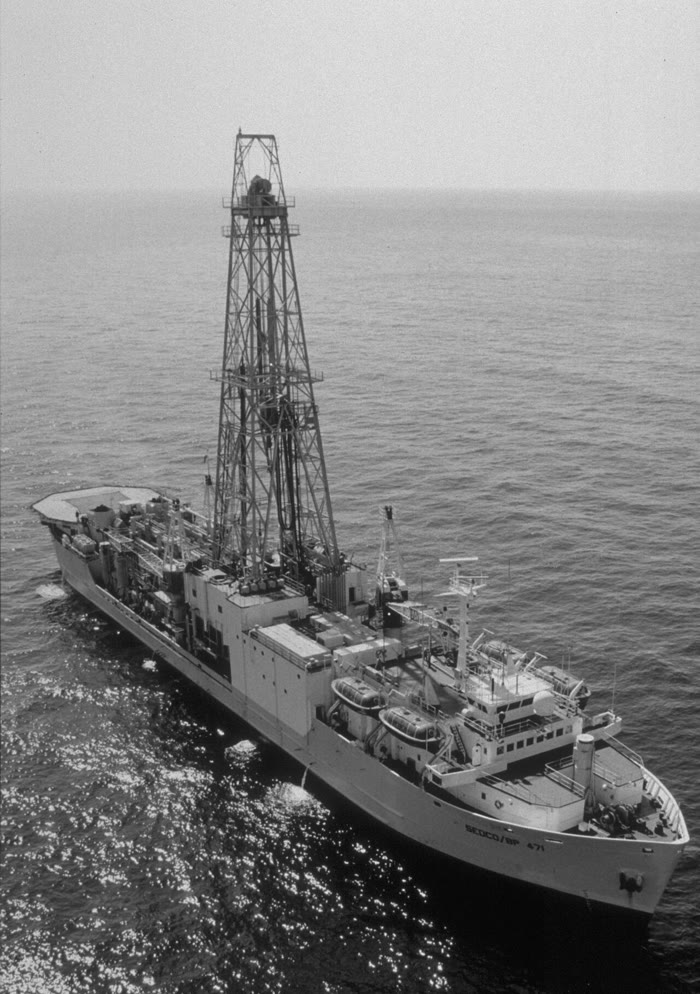
\includegraphics[width=0.36\linewidth]{images/book2/g11-odp-joides-resolution.jpg}

{\small El buque de perforación \emph{JOIDES Resolution}, sucesor del
\emph{Glomar Challenger}: la alta torre es su torre de perforación, y el
buque lleva más de \qty{9000}{m} de tubería de perforación. Fotografía: Ocean Drilling Program, Texas A\&M
University (dominio público).}
\end{omfigure}
% ledger: photo:g11-joides, usgs:glomar

Desde entonces, miles de perfiles magnéticos y cientos de sondeos se han
reunido en un mapa de la edad de todo el fondo oceánico.

\begin{omfigure}
\begin{tikzpicture}
\begin{axis}[ommap, width=\linewidth, xtick=\empty, ytick=\empty, grid=none,
    axis background/.style={}, clip=true, name=map]
  \addplot graphics[xmin=-180, xmax=180, ymin=-90, ymax=90] {figdata/out/grade-11-seafloor_age.png};
  \addplot[black!60, line width=0.15pt] table {figdata/out/shared-geo-land.dat};
\end{axis}
\begin{axis}[at={(map.south)}, anchor=north, yshift=-0.35cm, scale only axis, width=0.55\linewidth, height=0.32cm,
    xmin=0, xmax=200, ymin=0, ymax=1, axis y line=none, axis x line*=bottom,
    xtick={0,20,...,180}, tick label style={font=\scriptsize},
    xlabel={edad del fondo oceánico (millones de años); gris: sin fondo oceánico}, label style={font=\scriptsize},
    enlargelimits=false]
  \addplot graphics[xmin=0, xmax=200, ymin=0, ymax=1] {figdata/out/grade-11-seafloor_age-bar.png};
\end{axis}
\end{tikzpicture}

{\small La edad del fondo oceánico. Muy joven (rojo) a lo largo de las
dorsales, envejece al alejarse de ellas a ambos lados; el fondo más antiguo
(azul y morado) está en los bordes de los océanos, contra los continentes y
a lo largo de las fosas. Datos: Seton y colaboradores (2020), en celdas de
1 grado; contornos de las tierras: Natural Earth.}
\end{omfigure}
% ledger: data:b2-seafloor-age, data:ne-land (map computed in figdata/grade-11/seafloor_age.py)

El mapa lo confirma todo a la vez. A lo largo de cada dorsal el fondo es
joven, y su edad crece simétricamente al alejarse de ella. Ningún fondo
oceánico tiene más de unos \num{190} millones de años: el más antiguo está en
el Pacífico occidental y frente a la costa este de América del Norte (unas
pocas cuencas pequeñas del Mediterráneo oriental se cuentan aparte). La edad
media del fondo oceánico es de unos \num{64} millones de años, y alrededor de
tres cuartas partes tienen menos de 100 millones de años --- mientras que los
continentes conservan rocas mucho más antiguas. El
fondo oceánico es joven porque se fabrica sin cesar en las dorsales y, como
vio Hess, se destruye en otro lugar: dónde, es el tema del
\cref{ch:g11:subduction-zones}.
% ledger: data:b2-seafloor-age (oldest_open_myr 192.5, share_younger_100 0.76 in figdata/grade-11/seafloor_age.py), seton:mean-age, usgs:hess

\section{Ejercicios}

\begin{exercise}[$\star$]\label{exo:g11:drift-to-spreading:1}
Define la \omterm{def:g11:drift-to-spreading:spreading}{expansión del fondo oceánico}. ¿Cuál es la diferencia entre la
\omterm{def:g11:drift-to-spreading:spreading-rate}{velocidad de expansión total} y la semivelocidad de expansión de una dorsal?
\end{exercise}

\begin{exercise}[$\star$]\label{exo:g11:drift-to-spreading:2}
¿Por qué una lava solo registra la dirección del campo terrestre una vez que
se ha enfriado por debajo de unos \qty{580}{\celsius}? ¿Qué le ocurre a ese
registro si la roca se calienta después a \qty{700}{\celsius}?
\end{exercise}

\begin{exercise}[$\star$]\label{exo:g11:drift-to-spreading:3}
Una ecosonda oye el eco de su impulso \qty{5.2}{s} después de emitirlo.
Tomando como velocidad del sonido en el agua de mar \qty{1500}{m/s}, ¿a qué
profundidad está el fondo marino?
\end{exercise}

\begin{exercise}[$\star$]\label{exo:g11:drift-to-spreading:4}
En la escala de tiempo de polaridad de este capítulo: ¿cuánto ha durado el
intervalo normal actual? ¿Cuánto duró el episodio Jaramillo? ¿Cuántas
inversiones hubo en los últimos cinco millones de años?
\end{exercise}

\begin{exercise}[$\star$]\label{exo:g11:drift-to-spreading:5}
Las dorsales oceánicas tienen unos \qty{65000}{km} de longitud. La
circunferencia de la Tierra mide unos \qty{40000}{km}. ¿Cuántas vueltas a la
Tierra darían las dorsales?
\end{exercise}

\begin{exercise}[$\star\star$]\label{exo:g11:drift-to-spreading:6}
En un perfil magnético, el límite entre los intervalos Brunhes y Matuyama
(\num{0.78} millones de años) está a \qty{20}{km} del eje de la dorsal.
Calcula la semivelocidad y la velocidad total en centímetros al año.
\end{exercise}

\begin{exercise}[$\star\star$]\label{exo:g11:drift-to-spreading:7}
En otro perfil, el límite Gauss--Gilbert (\num{3.58} millones de años) está a
\qty{45}{km} al oeste y a \qty{44}{km} al este del eje. Calcula la
semivelocidad de cada lado y la velocidad total. ¿Es simétrica la expansión?
\end{exercise}

\begin{exercise}[$\star\star$]\label{exo:g11:drift-to-spreading:8}
El punto 19 de la perforación de 1968 está a \qty{990}{km} del eje de la
dorsal mesoatlántica. Con una semivelocidad de \qty{1.9}{cm} al año, predice
la edad del fondo allí, y compárala con los \num{49} millones de años de su
sedimento más antiguo.
\end{exercise}

\begin{exercise}[$\star\star$]\label{exo:g11:drift-to-spreading:9}
Una dorsal se expande con una semivelocidad de \qty{2}{cm} al año. Con la
escala de tiempo de este capítulo, da las distancias al eje de los límites de
0.78, 0.99, 1.07, 1.77 y 1.95 millones de años, y dibuja las bandas de un
lado, las normales en negro.
\end{exercise}

\begin{exercise}[$\star\star$]\label{exo:g11:drift-to-spreading:10}
La edad media del fondo oceánico es de unos \num{64} millones de años; la
Tierra tiene unos \num{4.6}~mil millones de años. ¿Qué fracción de la edad de
la Tierra es eso? ¿Qué argumento de Hess apoya?
\end{exercise}

\begin{exercise}[$\star\star$]\label{exo:g11:drift-to-spreading:11}
Explica, con un dibujo, por qué el dibujo de las bandas magnéticas de un lado
de una dorsal es la imagen especular del dibujo del otro lado. ¿Qué rompería
esta simetría?
\end{exercise}

\begin{exercise}[$\star\star\star$]\label{exo:g11:drift-to-spreading:12}
Supón que las dorsales, de \qty{65000}{km} de longitud en total, se expanden
a una velocidad total media de \qty{5}{cm} al año.
\begin{enumerate}
  \item ¿Qué superficie de fondo oceánico nuevo fabrican cada año, en
        \unit{km^2}?
  \item El fondo oceánico cubre unos \qty{2.9e8}{km^2}. ¿Cuánto tiempo
        tardarían las dorsales en fabricar esa superficie?
  \item Compáralo con el fondo oceánico más antiguo, de unos \num{190}
        millones de años. ¿Qué le tiene que ocurrir al fondo oceánico al
        mismo ritmo al que se fabrica?
\end{enumerate}
\end{exercise}

\begin{exercise}[$\star\star\star$]\label{exo:g11:drift-to-spreading:13}
El episodio Jaramillo duró de hace \num{1.07} a hace \num{0.99} millones de
años. ¿Qué anchura tiene su banda a cada lado de una dorsal con una
semivelocidad de \qty{1.25}{cm} al año, y de una con \qty{7.5}{cm} al año? La
roca magnetizada está a unos \qty{3}{km} por debajo de la superficie del mar.
Explica por qué el episodio se ve con claridad en el perfil rápido de este
capítulo y apenas en el lento.
\end{exercise}

\begin{exercise}[$\star\star\star$]\label{exo:g11:drift-to-spreading:14}
En los puntos de 1968, el sedimento tiene \qty{176}{m} de espesor en el
punto 16, cuyo fondo tiene unos \num{11} millones de años, y solo \qty{72}{m}
en el punto 20, de unos \num{67} millones de años. Calcula el ritmo medio al
que se acumuló el sedimento en cada punto, en metros por millón de años.
¿Puede usarse el espesor del sedimento para datar el fondo? ¿Qué se usa en
su lugar?
\end{exercise}

\begin{exercise}[$\star\star\star$]\label{exo:g11:drift-to-spreading:15}
En un perfil a través de una dorsal, el límite de \num{2.581} millones de
años está a \qty{58}{km} al oeste y a \qty{70}{km} al este del eje.
\begin{enumerate}
  \item Calcula la semivelocidad de cada lado y la velocidad total.
  \item El fondo al este del eje se fabricó más deprisa que el del oeste.
        Al cabo de 10 millones de años a estas velocidades, ¿a qué distancia
        del eje estaría el fondo de esa edad a cada lado?
  \item Explica por qué la distancia entre los dos límites da la velocidad
        total aunque la expansión no sea simétrica.
\end{enumerate}
\end{exercise}

\section{Problema: la edad del Atlántico Sur}

\begin{problem}[{Problema de fin de semana --- datar un océano de tres maneras}]
\label{pb:g11:drift-to-spreading:1}
% ledger: dsdp3:table5, dsdp3:rate, data:b2-seafloor-age, earth:Rmean, ics:base.Cretaceous
% (values computed in figdata/grade-11/sediment_ages.py and seafloor_age.py)
En 1968, el \emph{Glomar Challenger} perforó siete pozos a través de la
dorsal mesoatlántica cerca de la latitud \ang{30} S. La tabla da, para cada
punto, su distancia al eje de la dorsal, la edad del sedimento más antiguo
sobre el basalto (por sus fósiles) y, donde se identificó la banda de debajo,
la edad de esa banda magnética, en millones de años.

\begin{center}
\small
\begin{tabular}{|c|c|c|c|}
\hline
punto & distancia al eje (\unit{km}) & edad del sedimento más antiguo & edad de la banda magnética \\ \hline
16 & 191 & 11 & 9 \\ \hline
15 & 380 & 24 & 21 \\ \hline
18 & 506 & 26 & --- \\ \hline
17 & 643 & 33 & --- \\ \hline
14 & 727 & 40 & 38.5 \\ \hline
19 & 990 & 49 & 53 \\ \hline
20 & 1270 & 67 & 71 \\ \hline
\end{tabular}

{\small Datos: Deep Sea Drilling Project, Leg 3 (1970); las edades magnéticas
son el centro de los intervalos que allí se dan.}
\end{center}

\begin{center}
\begin{tikzpicture}
\begin{axis}[omrecord, width=0.82\linewidth, height=5.0cm, xmin=-50, xmax=16, ymin=0, ymax=140,
  xlabel={longitud a lo largo de \ang{30} S (grados; negativa: oeste)}, ylabel={edad (millones de años)},
  tick label style={font=\small}, label style={font=\small}, clip=false]
\addplot[omDef, line width=0.8pt] table[x=lon, y=age] {figdata/out/grade-11-seafloor_age-profile.dat};
\draw[omRidge, densely dashed] (axis cs:-13.8,0) -- (axis cs:-13.8,140);
\node[font=\scriptsize, text=omRidge, anchor=south] at (axis cs:-13.8,140) {eje de la dorsal};
\fill (axis cs:-47.4,125.1) circle (1.5pt);
\node[font=\scriptsize, anchor=south west, inner sep=2pt] at (axis cs:-47.6,126) {América del Sur};
\node[font=\scriptsize, anchor=north west, align=left] at (axis cs:14.2,135) {África};
\fill (axis cs:13.8,129.8) circle (1.5pt);
\end{axis}
\end{tikzpicture}

{\small La edad del fondo oceánico a lo largo del paralelo \ang{30} S, de
América del Sur a África; la línea se interrumpe donde el fondo oceánico
termina contra cada continente. Datos: Seton y colaboradores (2020).}
\end{center}

\medskip
\noindent\textbf{Parte I --- Los puntos de perforación.}
\begin{enumerate}
  \item ¿Qué punto está más cerca de la dorsal, y cuál más lejos? ¿Cómo son
        sus edades?
  \item ¿Por qué la edad del sedimento más antiguo que descansa sobre el
        basalto está cerca de la edad del propio basalto? ¿Es algo más
        antiguo o algo más joven?
  \item Para cada punto, calcula el cociente entre su distancia y la edad de
        su sedimento más antiguo, en kilómetros por millón de años.
  \item ¿Cuál es la media de estos siete cocientes? Conviértela a
        centímetros al año.
  \item Los puntos 17 y 18 están al este de la dorsal; los demás, al oeste.
        ¿Siguen los puntos del este la misma tendencia que los del oeste?
        ¿Qué dice eso sobre la expansión?
\end{enumerate}

\medskip
\noindent\textbf{Parte II --- La velocidad a partir de los sedimentos.}
\begin{enumerate}[resume]
  \item Si el fondo se hubiera expandido con una semivelocidad constante
        $u$, ¿cómo dependería la edad $t$ del fondo de su distancia $d$ al
        eje?
  \item La recta que pasa por el origen y mejor se ajusta a los puntos tiene
        la pendiente $u = \sum d\,t / \sum t^2$. Para los siete puntos,
        $\sum d\,t = \num{208276}$ y $\sum t^2 = \num{10952}$ (en
        kilómetros y millones de años). Calcula $u$ en kilómetros por
        millón de años y en centímetros al año.
  \item ¿Cuál es la \omterm{def:g11:drift-to-spreading:spreading-rate}{velocidad de expansión total} del Atlántico Sur a esta
        latitud?
  \item Los científicos de la expedición escribieron que la velocidad era
        ``algo menor de \qty{2}{cm} al año''. ¿Estás de acuerdo?
  \item Con esta velocidad, predice la edad del fondo en el punto 20, y
        compárala con su sedimento más antiguo.
\end{enumerate}

\medskip
\noindent\textbf{Parte III --- La velocidad a partir de las bandas magnéticas.}
\begin{enumerate}[resume]
  \item Solo a partir del punto 16 (\qty{191}{km}, banda de 9 millones de
        años), calcula una semivelocidad.
  \item Solo a partir del punto 20 (\qty{1270}{km}, banda de 71 millones de
        años), calcula una semivelocidad.
  \item Para los cinco puntos con edad magnética, $\sum d\,t = \num{180329}$ y
        $\sum t^2 = \num{9854}$. Calcula la mejor semivelocidad.
  \item ¿En qué porcentaje difieren las velocidades obtenidas con los fósiles
        y con las bandas? ¿Concuerdan los dos métodos?
  \item ¿Por qué es importante que las dos edades se obtuvieran por métodos
        completamente distintos?
\end{enumerate}

\medskip
\noindent\textbf{Parte IV --- Hasta el borde del océano.}
\begin{enumerate}[resume]
  \item A lo largo de \ang{30} S, el eje de la dorsal está a la longitud
        \ang{13.8} O, y el fondo oceánico termina contra África a
        \ang{13.8} E. ¿Cuántos grados de longitud los separan?
  \item En una esfera de \qty{6371}{km} de radio, un grado de longitud
        mide $\qty{111.2}{km} \times \cos(\text{latitud})$. Calcula la
        longitud de un grado a \ang{30} S, y la distancia del eje al borde
        del fondo oceánico junto a África.
  \item Si el fondo se hubiera expandido siempre a la velocidad de la
        Parte II, ¿hace cuánto tiempo se habría formado el fondo del borde?
  \item El mapa de edades, que data el fondo antiguo por sus bandas
        magnéticas, da \num{130} millones de años en el borde. ¿Qué
        semivelocidad media implica eso? ¿Fue la apertura temprana del océano
        algo más rápida o algo más lenta que la apertura de los últimos 66
        millones de años?
  \item Concluye: ¿qué edad tiene el fondo oceánico más antiguo junto a
        África a \ang{30} S? El periodo Cretácico empezó hace unos \num{143}
        millones de años: ¿en qué periodo empezó a abrirse allí el Atlántico
        Sur?
\end{enumerate}
\end{problem}
